%% Mẫu luận án tiến sĩ (thạc sĩ) theo style vietkey.luanan.1.2.cls - Version 1.2
%% (c) Dang Minh Tuan, Vietkey Group.
%% Tel: +84-98-868-6636, Email: tuanvietkey@gmail.com.
%%
%% History:
%% - version 1.2 (2017/08/11)
%% - Created on 2016/08/16.

\documentclass[fontsize=13pt,oneside,a4paper,openany]{vietkey.luanan.1.2}

%tham số firstinits=true để viết tắt, defernumbers để số thứ tự liền mạch.
\usepackage[backend=bibtex,
            bibstyle=luanan,
            sorting=nyvt,
            block=none,
            %defernumbers=true,
            babel=other]{biblatex}
\usepackage{titling}
\usepackage{setspace}
\usepackage{fancyvrb}
\usepackage{dirtytalk}
\usepackage{listing}

\addbibresource{../bibdmt.bib}                 %%% dữ liệu về tài liệu tham khảo.
\begin{document}

\begin{titlingpage}
\begin{singlespace}
% \calccentering{\unitlength}
% \begin{adjustwidth*}{\unitlength}{-\unitlength}

\begin{center}
{\Large \textsc{Vietnam National University \\Ho Chi Minh city University of Techonology}\\
\vspace{3mm}
Faculty of Computer Science and Engineering
}\\
\vspace{10mm}
% \vspace*{13mm}

\includegraphics[width=0.3\textwidth]{images/logo.png}\\
\vspace{1cm}
\rule[0.5ex]{\linewidth}{2pt}\vspace*{-\baselineskip}\vspace*{3.2pt}
\rule[0.5ex]{\linewidth}{1pt}\\[\baselineskip]
{\huge \textcolor{blue}{Windows Memory Forensics}}\\[4mm]
{\Large \textit{\textcolor{blue}{Finding hidden processes in running machine}}}\\
\rule[0.5ex]{\linewidth}{1pt}\vspace*{-\baselineskip}\vspace{3.2pt}
\rule[0.5ex]{\linewidth}{2pt}\\
\vspace{6.5mm}
{\large By}\\
\vspace{6.5mm}
{\Large\textsc{NGUYEN Anh Khoa - 1611617}}\\
\vspace{15mm}

\begin{minipage}{10cm}
A thesis proposal submitted to the Ho Chi Minh city University of Technology in accordance with the requirements of the degree of \textsc{Degree of Engineer} in Computer Science.
\end{minipage}\\


\vspace{10mm}
\begin{center}
\begin{tabular}{ r l }
\textbf{Instructors}:& \Large \textsc{NGUYEN An Khuong}\\
& \Large \textsc{NGUYEN Le Thanh}\\
& \Large \textsc{NGUYEN Quoc Bao}\\
\end{tabular}
\end{center}
\vspace{6mm}
{\large Ho Chi Minh city, \textsc{December 2019}}
\vspace{12mm}
\end{center}
% \end{adjustwidth*}
\end{singlespace}
\end{titlingpage}
                          %%% có thể thay đổi

\VKnumRoman                                 %%% đánh số bằng chữ cái i, ii...

% \include{loicamdoan}                        %%% có thể thay đổi
% \include{loicamon}                          %%% có thể thay đổi

\clearpage
% \addcontentsline{toc}{section}{\abstractname}
\begin{abstract}

Digital forensics is an action taken to extract raw data from computers and analyze that data to discover information or to learn about historical events that happened to the target machine. Computer forensics is more and more popular today where cyberattacks happen almost every day. When cyberattacks happen, we must stop the threat, but gathering information about the attack also has the same degree of importance. It is surprising how many information one can learn given only a snapshot of the memory, from running processes to hidden files and cryptographic keys. With high demands, people have come up with many techniques to analyze disk images, hard drives, and physical memory. No matter how great techniques we have for digital forensics, it is still worse than preventing an attack from happening. Even though Antivirus software, live reporting system and firewall mitigate some known attacks but with the new arising group of malware operate in stealth mode, like Cryptomining malware, or Rootkits remain a significant threat to organizations. In this paper, we would like to introduce a scanning system based on digital forensics to list running processes and to assist in the detection of malware.

\end{abstract}
\clearpage

\VKmucLuc                                   %%% mục lục

% \include{kyhieu}                            %%% có thể thay đổi

\VKdanhMucHinhVe                            %%% danh mục hình vẽ
\VKdanhMucBangBieu                          %%% danh mục bảng biểu
%\VKdanhMucDinhLy
%\VKdanhMucDinhNghia
\lstlistoflistings
\VKbatDaudanhSo                             %%% bắt đầu đánh số từ 1,2,3...

% \include{loinoidau}                         %%% có thể thay đổi
\chapter[Introduction]{Introduction}

In this chapter, we explain the definitions along with the current state of digital forensics and some contexts of today computer system and the current state we are in.

Before we get into the proposal, we shall understand the following terminologies as written below:

\begin{itemize}
  \item \textbf{Hacker}.
    Person who commits illegal activities to computer systems by exploiting bugs, or by writing illegal software that aims to damage or corrupt system, or by collecting sensitive, classified information.
  \item \textbf{Malware}.
    A type of computer software that does illegal activities such as stealing information; damaging or corrupting system; ransoming system owner; etc..
  \item \textbf{Trojans}.
    A type of computer software that collects computer information and activties without user's permission and/or acknowledgement.
    A digital asset used in place of cash or banking money, hardened by cryptographic security.
  \item \textbf{File signature}.
    Data used to identify or verify the content of a file. Commonly bytes in file and file checksum.
\end{itemize}

\section[Motivation]{Motivation}

Throughout the years of computer development, computers have become a standard method for humans around the world to study, work and entertain. Most activities of our daily lives involve computers. Individuals across the globe have created systems running on computers to assist them in doing common and complex tasks. However, this somehow influenced other people to commit harmful activities. Hackers have been creating malware damaging and stealing information. Furthermore, lately along with the trend of cryptocurrency, while ordinary people commit their investment by using crypto mining machines, hackers, on the other hand, create sophisticated malware (cryptojacking malware) that stealthily installed on a victim machine and mine cryptocurrency without the victim's acknowledgement.

Security researchers have been struggling to find ways to mitigate the gaining rate of attacks. However, it was never close to perfection. We rely on file signature database for filtering and often miss out new one, thus, it is highly vulnerable to the newer class of malware. To counterattack these new malware, we perform digital forensics when an attack happens. Digital forensics which as described by The Forensics Research Workshop I \cite{roadmap}:

\say{The use of scientifically derived and proven methods toward the preservation, collection, validation, identification, analysis, interpretation, documentation and presentation of digital evidence derived from digital sources for the purpose of facilitating or furthering the reconstruction of events found to be criminal, or helping to anticipate unauthorized actions shown to be disruptive to planned operations.}

% https://www.mcafee.com/enterprise/en-us/assets/infographics/infographic-threats-report-dec-2018.pdf
% https://www.mcafee.com/enterprise/en-us/assets/reports/rp-quarterly-threats-aug-2019.pdf

Digital forensics includes many different aspects, however, the most intrigued part of digital forensics is memory forensics, which "provides unprecedented visibility into the runtime state of the system, such as which processes were running, open network connections, and recently executed commands" as stated in the book The Art of Memory Forensics \cite{ligh2014art}. Not only can we get a frame of a computer state, but we can extract files and processes which was in the memory. If we can identify a malware, we can extract them and learn the malware behaviour through traces in the system. Then we reverse engineer the malware and create its signature and add to our database.

A malware is good only before it is discovered, therefore hackers creates malware hidden from the Task Manager. From the early days of 1990s, hackers have been improving ways to hide malware. In 2017, a small report \cite{evolutionHidding} have revised hiding techniques in malware over the years in Windows OS. [NEED THE PAPER CONCLUSION]. Even in 2019, we can still observe incidences where malware hide itself so effective. For example, an Android malware that hid themselves on user mobile and was only found September 2019 after 5 months on the Google Play Store \cite{hiddenMalwareAndroid}, or the Titanium backdoor\footnote{Programs that receives remote connections} on Windows 10 disclosed November 2019 \cite{titanium}, or the macOS malware, unioncrypto, that download and run a hidden process in memory to mine cryptocurrency was found out December 2019 \cite{unioncrypto}. Researchers collected and analyzed these malware, but a normal user would not be able to do that. For a normal user, if the anti-virus software failed to flag the file as mallicious, his computer will be infected. To know whether a system is having a hidden malware running, we must extract the memory and send to an investigator to find out. Such process is complex, long and costly, a user must know how to extract the memory and hire an investigator to analyze. Another way is to do memory forensics live \footnote{when the system is still running} and automatically extract and send the hidden process binary to the researchers. Shuaibur Rahman and Khan \cite{reviewLive} has a review of live forensics analysis techniques in 2015, one standout paper is \cite{comparativeLive} described the technique to find finished and cache\footnote{background running processes} processes. However, the paper is only restricted to the Linux OS. Others approaches mentioned uses memory acquisition technique to get the memory dump and perform analysis later. There are projects that implements memory forensics techniques but is limited to dump file analysis. We have researched for live memory analysis and have come up with a method for finding hidden processes.

Our target has some requirements, it must be easy to use for normal user, and target Windows 10. The market share of Windows over others OS is higher \cite{osMarketShare}, within the Windows OS, version 10 is now dominating \cite{windowsShare}, also high level of malware targeting Windows has convinced us to set the target to Windows 10. The outcome of this project will be a small tool searching and collecting hidden processes and sending the process binary to the server.

\section[Objectives]{Objectives}

In the scope of this proposal, we wish to:

\begin{itemize}
  \item Understand the basics concept of OS that supports memory forensics.
  \item Understand to some extend the internal of Windows operating system.
  \item Understand some techniques often use for analyzing Windows memory dump.
  \item Analyze some already exists tools support for memory forensics.
  \item Propose a method to find hidden running processes in running Windows machine.
\end{itemize}

\section[Structure]{Structure}

% TODO


\chapter[Background]{Background}
\section[Operating system concepts]{Operating system concepts}

\subsection[Multiprogramming]{Multiprogramming}

Multiprogramming defines a computer where it can run serveral programs simutaneously. To enable multiprogramming the OS must be capable of managing memory region for processes, scheduling running time for processes, and many more crucial tasks. We will briefly review the two aspect of multiprogramming.

The first aspect is scheduling. Cooperative multitasking, or so called non-preemptive multitasking, is a design for multiprogramming scheduling where it does not limit a process's runtime. A process will actively run until it stops/idles or waits for an I/O operation, whence the operating system will change (switch context) to another process. In contrast with cooperative multitasking, preemptive multitasking limits the process's runtime and initiate a context switch when either the time alloted is used or the process waits for an I/O operation. Both schemes have been used in many operating systems but cooperative multitasking schema is not suitable for multiple usage OS, thus in most modern operating system for general usage (Windows, MacOS, and most Linux distributions), preemptive multitasking schema is chosen.

\begin{figure}
  \centering
  \caption{Preemptive}
  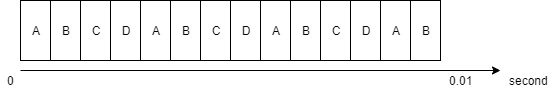
\includegraphics[scale=0.8]{images/preemptive.png}
  \text{4 processes (A, B, C, D) running in a tiny time slot which appears simutaneously to a human}
\end{figure}

The second aspect is memory management. In the early days, memory management was so simple that it would contain the whole process consecutively in memory. However, doing this leads to external fragmentation, where the memory is empty but not fit consecutively for a process Figure~\ref{fig:externalfragmentation}. OS developers soon realize storing the whole process in memory is not optimize when programs only need a part of memory at a specific time when running. They came up with ways to load only the necessary parts in memory. After many years, people have agreed upon splitting a process to equal parts called a \textit{page}. The OS splits the physical memory to pages and load processes data to those pages Figure~\ref{fig:splitprocess}. When a process needs more space or needs parts that are not on the memory, the OS will find an empty/unused page to load in. If there is no empty page, one least use page will be moved (swapped out or page out) to disk to make space. The OS tracks what pages a process is using and swap those pages in and out by process need.

So far, we have only discussed processes that have a limited amount of memory, but the OS allows programs to have more space by using the paging technique describe above. Because process data can be moved to disk and brought back when needed, a process can have as many space as the disk space available. However by most OS implementation, a process should have a limited virtual address space. Because the address is virtual to the process, every memory access will need the OS to change to the address in the physical memory (after page swapping). Changing address from virtual to physical is called \textit{address translation}. By using virtual memory, the OS can map the same data to many processes and reuse data. For example, two processes use the same library in Figure~\ref{fig:samelib}.

Example for address translation. Assuming the OS allows a process to have 2GB of (virtual) memory space (from 0 to $2^{32}-1$), and a page will have the size of 4KB, and the system have 4GB of physical memory. A process loading at 0x40000000 will have all data from 0x40000000 to (0x40000000 + 4KB) loaded to physical memory at the address of 0x60000000 to (0x60000000 + 4KB).

\begin{figure}
\centering
\caption{External fragmentation}
\label{fig:externalfragmentation}
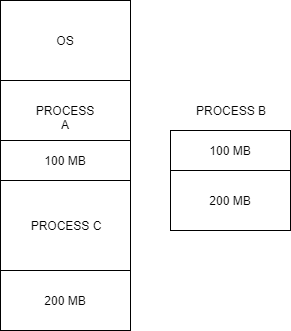
\includegraphics[scale=0.5]{images/external_fragmentation.png}
\end{figure}

\begin{figure}
\centering
\caption{Splitting process}
\label{fig:splitprocess}
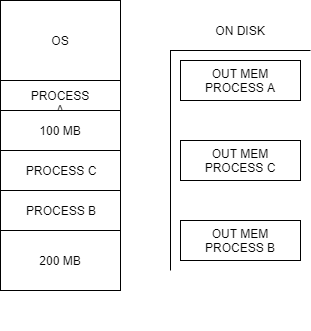
\includegraphics[scale=0.5]{images/splitting_process.png}
\end{figure}

\begin{figure}
\centering
\caption{Splitting process}
\label{fig:samelib}
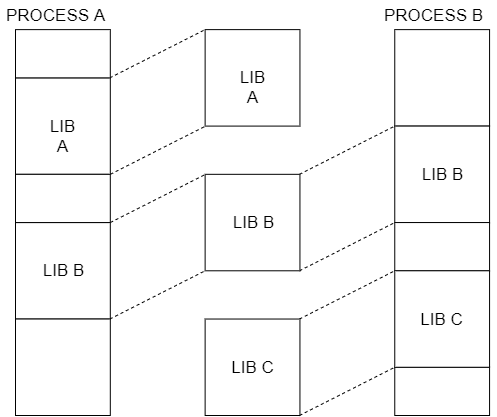
\includegraphics[scale=0.5]{images/use_same_lib.png}
\text{Two processes use the same library (LIB B) and is visible in its own (virtual) address space}
\end{figure}

\section[Windows Internals]{Windows Internals}

Windows is a widely used Operating System; it was first designed for non-IT people in the industry and luckily stood out to the crowd. People started buying Windows for their job. The market soon rocketed and almost everywhere uses Windows as their primary OS to work or study. Even when macOS and Linux are becoming more popular nowadays, Windows market share of Desktop OS is still more than 75\% \cite{windowsStat}. With a vast majority of Windows as the primary OS, malware targeting Windows is therefor higher. According to statista.com, in the first quarter of 2019, 74.49\% of malware detected is aiming for Windows \cite{windowsMalwareStat}. Because Windows will still be the most used OS by users and the most targeted OS by hackers in the future, this is the reason why we have taken Windows memory analysis as our primary focus throughout the paper. In this section, we will discuss some Windows Internals in advance of memory forensics details next section.

\subsection[Memory model]{Memory model}

We start by exploring the Windows memory model. Windows by default use page size of 4KB, the address space for each process is 2GB for the 32-bit version and 8TB for the 64-bit version. The system address space is 2GB for the 32-bit version and 248TB for the 64-bit version. Every process, when run, can see its own address space and system space too, but access to system space is restricted. A typical 32-bit process can have a 2GB space for itself and a 2GB space of the system, makes a total memory space 4GB. The system space (kernel space) contains the OS and the currently running drivers. In this space contains items that specify the current state of the OS. The kernel space uses \textit{pools} to manage structures' allocation and deallocation. Windows has two types of pool, one that is \textit{pagedable} called \textit{paged pool} and the other \textit{non-paged pool}. The size of these two types of pool on Windows 10 can be reference through the table~\ref{tab:poolsize} \cite{memorylimit}. Because many parts of the OS is not used often, Windows can swap those pages out to make more space. However, critical information, including processes' information, is stored in non-paged pools.

\begin{center}
\begin{table}[h]
\begin{tabular}{|l|p{5cm}|p{5cm}|}
\hline
Pool Type & Limit on 32-bit & Limit on 64-bit \\ \hline
Paged Pool & 384 GB or system commit limit, whichever is smaller & 384 GB or system commit limit, whichever is smaller \\ \hline
Non-paged Pool & 75\% of RAM or 2 GB, whichever is smaller. & RAM or 128 GB, whichever is smaller (address space is limited to 2 x RAM) \\ \hline
\end{tabular}
\caption{Pool size on Windows 10}
\label{tab:poolsize}
\end{table}
\end{center}

The memory pool is a bitmap\footnote{An array of bits}. Windows will return the pointer and size when asked for space in the pool. Windows keeps track of chunks in the pool. At first, there is only one chunk (the pool itself). When the user asks for space, Windows will split the chunk to two, one for the user and one left unused, Windows will split the unused space in pool and return to the user for any allocation requested. Upon deallocation, Windows will merge unused chunks into one. Consider the code in Listing~\ref{lst:basicpool} for a basic example of pool allocation.

Each chunk will have a \texttt{POOL\_HEADER} field on top to denote the content of the chunk. \texttt{POOL\_HEADER} has a size field (\texttt{BlockSize}), a previous size field (\texttt{PreviousBlockSize}), and a tag (\texttt{POOL\_TAG}). Tag is a four-byte character that Windows and Driver writer use to denote the data stored in the chunk. The typical description of \texttt{POOL\_HEADER} is at Listing~\ref{lst:poolheader}. In Table~\ref{tab:pooltag}, we listed some typical structure with its tag.

\lstinputlisting[language=C,caption={POOL\_HEADER},label={lst:poolheader},basicstyle=\linespread{0.8}]{code/poolheader.cpp}

\lstinputlisting[language=C,caption={Basic Pool Algorithm},label={lst:basicpool},basicstyle=\linespread{0.8}]{code/basic_pool.cpp}

\begin{center}
\begin{table}[h]
\begin{tabular}{|l|l|l|}
\hline
Structure     & Structure Name   & Pool Tag \\ \hline
Driver Object & \_DRIVER\_OBJECT & Driv     \\ \hline
File Object   & \_FILE\_OBJECT   & File     \\ \hline
Process       & \_EPROCESS       & Proc     \\ \hline
TCP endpoint  &                  & TcpE     \\ \hline
TCP listener  &                  & TcpL     \\ \hline
Thread        & \_ETHREAD        & Thre     \\ \hline
UDP endpoint  &                  & UdpA     \\ \hline
\end{tabular}
\caption{Some pool tag and corresponding structure}
\label{tab:pooltag}
\end{table}
\end{center}

\subsection[EPROCESS]{EPROCESS}

Windows has a special structure that contains a process information called \texttt{\_EPROCESS}. This structure is created every time when a new process spawn and located inside a non-paged pool with tag \textit{Proc}. If we have a reference to one \texttt{\_EPROCESS} we might follows \texttt{LIST\_ENTRY ActiveProcessLinks} (a doubly linked list pointer) to find other \texttt{\_EPROCESS} of different process. However because this structure can be accessed by a normal user by calling \texttt{PsLookupProcessByProcessId} one may edit the doubly linked list to remove itself from the list chain. This is called \textit{DKOM} (Direct kernel object manipulation) and is used very often in malware to hide itself from process explorer. With the given \texttt{LIST\_ENTRY} structure in \ref{lst:listentry}, refrence the graphics \ref{fig:eprocesslink} and \ref{fig:dkom} that explains the normal EPROCESS linking and DKOM.

\begin{lstlisting}[language=c,caption={LIST\_ENTRY},label={lst:listentry}]
typedef struct _LIST_ENTRY {
      struct _LIST_ENTRY *Flink;
      struct _LIST_ENTRY *Blink;
} LIST_ENTRY, *PLIST_ENTRY, PRLIST_ENTRY;
\end{lstlisting}

\begin{figure}
\centering
\caption{EPROCESS Linking}
\label{fig:eprocesslink}
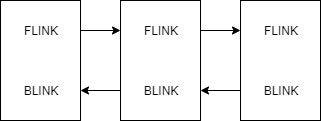
\includegraphics[]{images/eprocess_link.png}
\end{figure}

\begin{figure}
\centering
\caption{DKOM}
\label{fig:dkom}
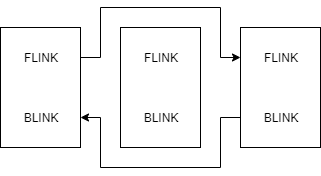
\includegraphics[]{images/dkom.png}
\end{figure}

\subsection[KDBG]{KDBG}

KDBG short for \texttt{Kernel Debugger Block} is one of commonly used structure when analyzing a memory artifact of Windows. It was created to easy debugging process for developers when writing OS or kernel drivers. As this struture contains pointers to others structures. One pointer contained in KDBG is \texttt{PsActiveProcessHead} which is a pointer to an \texttt{\_EPROCESS}. As previously mentioned, we can walk the list of \texttt{\_EPROCESS} to enumerate all processes.

However from Windows 8, this structure is encoded and hinders us from analyzing windows memory. As quoted by the developers of Volatility \cite{kdbgEncoded},

\say{An encoded KDBG can have a hugely negative effect on your ability to perform memory forensics. This structure contains a lot of critical details about the system, including the pointers to the start of the lists of active processes and loaded kernel modules, the address of the PspCid handle table, the ranges for the paged and non-paged pools, etc. If all of these fields are encoded, your day becomes that much more difficult.}

Why users of Volatility will suffer a bad day, Rekall's users do not as they use another method without knowledge of KDBG structure \cite{rekallOnKDBGEncoding}. However, KDBG is still an important Windows structure that provides kernel information.

\subsection[Windows dump file]{Windows dump file}

Windows provides a dump file to contains compressed memory data. This file is created by Windows when an error in kernel occur. Third party tools can dump the memory on running machine for example, DumpIt, FTK Imager. This file structure is not documented, however, it was written on Microsoft debug file, Schuster \cite{dmpfile} has written a guide to the file structure. Another dump file type is mini dump file which is documented by Joachim \cite{mdmpfile}. These dump files are commonly used to preserve the system memory state for analysis.

\section[Digital Forensics and memory forensics techniques]{Digital Forensics and memory forensics techniques}

Digital forensics describes the process includes the collection and analyzation of evidence; information synthesization; and sometimes unknown binaries and files analysis. Digital forensics has become significant in the industry. People will turn into digital forensics companies when they notice or doubt one computer contains illegal files or malicious applications. Without digital forensics, we cannot traceback when an attack happens, and without prior learning of historical events, we can not build a more reliable system to detect and prevent future replicate attacks. We learn and build filters based on files signature \cite{yararules}. These signatures can be unknown from a Zero-day attack, and even a One-day attack can still harm the system. Digital forensics is gaining more and more important when the next generation of malware do not intend to break the system but to exploit the system computing power for profit or collect sensitive information. Most notably are Cryptocurrency Malware and Botnet; these types of malicious applications will run inside the system and uses little computations. Backdoors and trojans are another concern when they silently collect user's information, files and activities. We can only know of their existence when the attack had happened.

\subsection[Evidence gathering]{Evidence gathering}

Once we have identified the corrupted system, we must try to disconnect the machine from the internet. However, if we disconnect the system from the internet, the malware will drop all connection, and we will lose all traces. Hence, we must quickly dump the memory of the system and disconnect the machine from the internet. An investigator can collect the information below from a memory dump.

\begin{itemize}
% \setlength\itemsep{-0.5em}
\item Currently running processes
\item Currently opening files (file descriptor)
\item Currently opening sockets
\end{itemize}

After memory dump file acquisition, we use forensics tools and begin analysis. In the worst condition, where we must shut down the system, we can try to collect the whole physical memory by using \textit{cold boot attack} \cite{coldboot}. This technique relies on memory data dissolve slower on low temperature, enable us to shut down and collect RAM data given physical access. Full RAM dump can easily be converted to dump file format to use with tools. After raw memory is gathered, we will start analyzing. The two go-to tools for memory forensics are Google's Rekall platform and the open-source Volatility project. Most digital forensics individuals and teams use these two tools. Next, we will describe some techniques on memory forensics.

\subsection[KDBG scanning]{KDBG scanning}

Scanning KDBG will provide some small but important piece of information. As described in Section ~\ref{sec:kdbg}, KDBG has a member \texttt{PsActiveProcessHead}, which is a pointer to the doubly linked list of \texttt{\_EPROCESS}. Volatility used KDBG scanning to characterize Windows version before Windows 8. From Windows 8 forward, this structure is encoded and made a hindrance to Volatility users \cite{kdbgEncoded}.

\say{An encoded KDBG can have a hugely negative effect on your ability to perform memory forensics. This structure contains a lot of critical details about the system, including the pointers to the start of the lists of active processes and loaded kernel modules, the address of the PspCid handle table, the ranges for the paged and non-paged pools, etc. If all of these fields are encoded, your day becomes that much more difficult.}

While users of Volatility will suffer a bad day, Rekall's users do not as Rekall uses another method without the knowledge of KDBG structure \cite{rekallOnKDBGEncoding}. However, KDBG is still a critical Windows structure that provides kernel information and still being used to get general information of Windows out of a dump file.

\subsection[Pool tag scanning and quick scanning]{Pool tag scanning and quick scanning}
\label{sec:pooltagscanning}

Pool tag scanning was first introduced by Schuster \cite{pooltagscan} in 2006. By utilizing the pool layout with \texttt{POOL\_HEADER}'s \texttt{POOL\_TAG}, scanning for tags that contain a certain structure is possible. With the larger physical memory in these recent years, scanning the whole address space will soon unsuitable. In 2016, Sylve, Marziale and Richard \cite{sylve2016pool} has improved the algorithm for 64-bit Windows by using a global kernel variable indicating the start of dynamic allocation of the pool \texttt{MiNonPagedPoolStartAligned} and a pointer to the allocation bitmap \texttt{MiDynamicBitMapNonPagedPool}. Their work has been proven to be much faster and work effectively on huge memory. Even today, pool tag scanning is still being used often to identify structure not found by the kernel structure indexing. Thus, pool tag scanning is used to search for hidden processes by finding \texttt{\_EPROCESS} that are not found by traversing the list of \texttt{\_EPROCESS}.


\chapter[Related works]{Related works}

\section[Volatility]{Volatility}

Volatility is an open-sourced forensic tools first developed by Aaron Walters and Petroni. It was first introduced in 2000 and by now Volatility has gain much popular in the digital forensics world. This work combines years of digital research into a convenient and versatile tool. The tool allows forensics investigators to analyze a memory dump file of Windows, macOS and Linux. It is designed by plugins of different version of OS, includings major, minor and build version. These plugins specify constatnt numbers, kernel structure definitions and others OS related information.



\section[Rekall]{Rekall}


\chapter[The proposed method]{The proposed method}

With the pool tag scanning described in section \ref{sec:pooltagscanning}, we proposed a way to do it live. The steps are listed below for clarity:

\begin{enumerate} % [label={Step \arabic.*}]
  \item Run a process in kernel mode
  \item Get a pointer to an address in the non-paged pool, and peform pool tag scanning
  \item Deserialize the bytes
  \item Collect information, compare with a legitimate list of \texttt{\_EPROCESS}, and send to the server
\end{enumerate}

Our program should have two parts, part that runs inside the kernel space, \texttt{K}, and part that run in user space, \texttt{U}. We will perform pool tag scanning with \texttt{K} and for every successful findings, \texttt{K} will send the structure as bytes to \texttt{U}. From that \texttt{U} will try to extract information by deserialize the bytes to a defined structure.

\section[Step 1]{Step 1}

Since our target is to seek structures that represent information of arbitrary structure of data in the kernel space, we should benefit from a driver running in kernel mode. There are two typical ways to run a driver in kernel mode. We can register the driver to run when Windows starts or manually load the driver when we need. Both ways need us to have a key in the registry of Windows at \texttt{\textbackslash registry\textbackslash machine\textbackslash SYSTEM\textbackslash CurrentControlSet\textbackslash Services}. The key must contains these three value:

\begin{itemize}
  \item \textbf{ImagePath}: the path of the driver to be loaded
  \item \textbf{Start}: enumeration specifing when to start the driver, manualy or on boot
  \item \textbf{Type}: enumeration specifing the type of the driver/service
\end{itemize}

Some enumeration we would use for \textbf{Start} are:

\begin{itemize}
  \item 2: Automatically. Started by \textit{smss.exe}
  \item 3: Manually.
  \item 4: Disabled.
\end{itemize}

For the \textbf{Type}, we will use \textit{1} as it specify a \texttt{kernel device driver}. If we want to manually load the driver, we should call the undocumented Windows API \texttt{NtLoadDriver(PUNICODE\_STRING RegistryPath)} with the \texttt{RegistryPath} is the registry key has the \texttt{ImagePath} is the path of the driver we want to load, \texttt{Start} set to \textit{3}, and \texttt{Type} is \textit{1}. When all is done, we now have a driver running in the kernel mode, which has access to the kernel space. Then we will proceed to find an address in the pool.

\section[Step 2]{Step 2}

Step two is when we find an address to a non-paged pool. We should be very careful when accessing the kernel space because the kernel is very sensitive to bad memory access. If we accidentally dereference an invalid address\footnote{address which does not have a backed up page}, we will get a kernel error, and either the driver stops or the system stops. To get an address in the pool we could either start scanning from \texttt{MiNonPagedPoolStartAligned} or request a chunk using \texttt{ExAllocatePoolWithTag(POOL\_TYPE PoolType, SIZE\_T NumberOfBytes, ULONG Tag)}. The \texttt{ExAllocatePoolWithTag} API will allocate a pool with \texttt{NumberOfBytes} size with type as \texttt{PoolType} and the tag \texttt{Tag}. If we call the API with \texttt{PoolType} \texttt{NonPagedPool}, we will have a chunk inside a non-paged pool. After we have a chunk inside a non-paged pool, we can perform pool tag scanning for \texttt{\_EPROCESS}.

When we found a potential \texttt{\_EPROCESS}, we capture the bytes based on \texttt{BlockSize} and send back to the user mode process \texttt{U}. After \texttt{U} receives the bytes, it will deserialize to the struct.

\section[Step 3]{Step 3}

To deserialize the bytes, we need the structure definition, however, Windows structures change drastically over builds \cite{windowsKernelCharacterization}. Thus, \texttt{\_EPROCESS} can have different members, or members' offset different across Windows build. Because many driver writters use kernel structures, it becomes difficult for them to debug when structures is not fixed. To help driver developers debug, Windows uses the \textit{PDB} (program database) file, a kind of file containings build information of a specific Windows version. These files can be downloaded online and is used by Windbg\footnote{A Microsoft debugger} and Visual Studio. We will use these files to get the precise structure definition of \texttt{\_EPROCESS} of the current Windows build we are running the tool on.

The PDB file has no official definition of the file layout, however Windows did provide us a repository containing information about this file type, though incomplete \cite{microsoft-pdb}. Many open-sourced tools have been created to parse these PDB files, we can create our own parser base on these. Before we parse the file, we should download the file first. All the PDB files is stored online on the Microsoft server, however, the server does not use HTTP as the download method. We must use either use Windbg or use a PDB-downloader tool created by Rajkumar Rangaraj \cite{pdb-downloader}. With these information, we can create a downloader and parser of PDB file to get the \texttt{\_EPROCESS} structure definition.

\section[Step 4]{Step 4}

After we have parsed the PDB file and the correct structure for \texttt{\_EPROCESS}, we can collect useful information such as process id, process create time, file path. The type and variable name of the information is as follows:

\begin{itemize}
  \item \textbf{Process id}: \texttt{PVOID UniqueProcessId}
  \item \textbf{Process create time}: \texttt{LARGE\_INTEGER CreateTime}
  \item \textbf{File path}: \texttt{UCHAR ImageFileName[16]}
\end{itemize}

We notice that \texttt{UniqueProcessId} field is a pointer, which we should ask the driver \texttt{K} to dereference it. Other than that, we should be able to get processes running in our system through pool scanning technique. We then traverse the doubly linked list \texttt{LIST\_ENTRY ActiveProcessLinks} in a normal process \texttt{\_EPROCESS}, which we can get by calling \texttt{PsLookupProcessByProcessId}\ref{lst:pslook}, to see if there is any difference. If there is a process found by pool tag scanning, and not present after traversing the \texttt{ActiveProcessLinks}, we flag the file as malicious.

After we have a list of \texttt{\_EPROCESS} that is malicious, we will try to get the binary file and the process memory. Both information is very usefull to analyze the file. From the \texttt{ImageFileName}, we can get the binary file, if we cannot get the file, we can still dump the memory of the process. Geoff McDonald \cite{processdump} has created a tool to dump a process by its process id, we can use the same method to dump the binary perfectly\footnote{The dumped binary is reconstructed in a readably/executable way}. After that, we will send all the dump binary files to the server for furthur analysis.

\begin{lstlisting}[language=c,caption={PsLookupProcessByProcessId},label={lst:pslook}]
NTSTATUS PsLookupProcessByProcessId(
  HANDLE    ProcessId,
  PEPROCESS *Process
);
\end{lstlisting}

\section[Evaluation]{Evaluation}

The proposed method uses pool tag scanning, so we should face the same problems by doing pool tag scanning. We may find a \textit{deleted} or \textit{freed} process. Or when some part of RAM could not be cleaned on shutdown\footnote{The cold boot attack mechanism}, some processes may have their \texttt{CreateTime} before the system start time. Also, the process starts scanning and send the binary only, which is half the information needed for investigation. The missing piece of information is process activities, but we do not monitor the system. For better information gathering, we should add in monitoring feature which is not the scope of this project. Another thing we may consider is scanning alone for \texttt{\_EPROCESS} could lose some potential malware that hides by memory execution. Some malware will create a thread in other process by using \textit{DLLL injection}, this case there will be no \texttt{\_EPROCESS} but \texttt{\_ETHREAD} is created. We could extend our tool to search for \texttt{\_ETHREAD} but that should be left after the proof of concept of scanning for \texttt{\_EPROCESS}. This method also only discuss on pool tag scanning and does not use pool tag quick scanning \ref{sec:pooltagscanning}, for a big memory system, this could result in long scanning time. Pool tag quick scanning should be an improve, but we will focus on implementing the plain pool tag scanning technique.

% \include{ketluan}                           %%% có thể thay đổi
% \include{chdanhmuccongbo}                   %%% có thể thay đổi

\nocite{*}
\VKngatTrang                                %%% ngắt trang để chuyển sang tài liệu tham khảo
\VKtaiLieuThamKhao                          %%% tài liệu tham khảo
\VKdanhSoPhuLuc                             %%% bắt đầu đánh số cho phụ lục

% \include{phuluccaidat}                      %%% có thể thay đổi

\end{document}

